
Como parte simplificada de la estructura de una comunidad de nodos en una red social, cada uno representa a un individuo y la red tiene una segmentación multitudinaria~\cite{ma2014exploring}. Algunas personas son centrales en la comunidad, algunas están al margen, establecen menos relaciones con otros y, por lo tanto, tienen una influencia menor. En esta sección, presentamos un nuevo enfoque de descubrimiento comunitario basado en el algoritmo PageRank para encontrar a estos delincuentes ``importantes" ó con ``mayor influencia" en nuestro grafo, con el fin de analizar supuestas bandas delictivas.
Recordemos que un grafo es un par $G = (N, A, g)$ donde $N$ es un conjunto finito no vacío de elementos denominados \textit{nodos} (vértices), $A$ es un conjunto de arcos y $g$ es una función que asocia a cada arco $a$ perteneciente a $A$ con un par no ordenado $(x, y)$, siendo $x$ e $y$ nodos pertenecientes a $N$. Se dice que $a$ es un arco con vértices extremos $x$ e $y$~\cite{dubinsky1984mathematical}.
%\vspace{-10pt}

\subsubsection{PageRank}
(PR) es un método que fue implementado a través de un algoritmo
originalmente utilizado por Google que asigna a cada página web de un conjunto dado, un puntaje que refleja su importancia dentro del conjunto. A este puntaje se lo denomina \textit{valor de PageRank}. Ante una consulta, el buscador utiliza estos puntajes para determinar el nivel de relevancia de las páginas, y retorna en primer lugar aquellas con un puntaje más alto. Para calcular los puntajes, PageRank utiliza la estructura de enlaces de la web~\cite{brin1998anatomy}. Una página web tiene un valor de PageRank alto si es apuntada por muchas otras páginas, o bien si es apuntada por páginas con puntajes altos~\cite{page1999pagerank}. PageRank tiene una base intuitiva en el concepto de \textit{random walks} sobre grafos~\cite{gobel1974random}: supongamos que un navegante aleatorio empieza a navegar la web desde una página cualquiera. El navegante puede hacer clic en forma aleatoria sobre alguno de los enlaces presentes en la página en la que se encuentra actualmente con una probabilidad $d$ a la que se denomina \textit{damping factor}, o bien con probabilidad $1-d$ accede aleatoriamente a cualquier otra página web. Este proceso se repite indefinidamente. Luego, el valor de PageRank de una página $P$ puede ser interpretado como la probabilidad de que el navegante aleatorio se encuentre en $P$ al finalizar el proceso. PageRank es definido formalmente de la siguiente manera ~\cite{franceschet2011pagerank}. Sean $q_i$ el número de enlaces salientes que posee la página $i$ , $n$ el número total de páginas web, $d$ el \textit{damping factor} que por lo general adquiere el valor 0.85, $\pi$ un vector columna denominado \textit{vector PageRank}, y $H = (h_{ij})$ una matriz cuadrada de tamaño $n$ tal que $h_{ij} = 1/q_i$ si existe un enlace desde la página $i$ a la página $j$ , y $h_{ij} = 0$ en caso contrario. El valor $h_{ij}$ corresponde a la probabilidad de acceder a la página $j$ desde la página $i$ en un paso, a partir de hacer clic en alguno de los enlaces que aparecen en esta última. El valor de PageRank correspondiente a la página $j$ es $\pi_j$, y se define recursivamente como se muestra en la ecuación \ref{eqn:ecuacionPageRank}~\cite{lin2010data}.
%\vspace{-5pt}

\begin{equation} 
	\label{eqn:ecuacionPageRank} 
	\pi_j = \frac{1-d}{n} + d \sum_{i=1}^{n} \pi_i h_{ij} 
\end{equation}
%\vspace{-20pt}

\subsubsection{Aplicación de PageRank para bandas delictivas}
Nuestro dataset descrito anteriormente se obtiene a partir de consultas SQL a la Base de Datos de \texttt{Coirón}. Para hacer uso del algoritmo de PageRank se decidió incorporarlo dentro de esas consultas SQL de modo de obtener un resultado que pueda ser utilizado para la visualización. Dentro de la consulta original se genera una tabla para los nodos y otra tabla para las relaciones, de esta manera el software realizado para la visualización obtiene dichos datasets y renderiza el grafo.
Para incorporar el cálculo de PageRank, inicialmente se adecuaron ambas tablas para la utilización de la fórmula, y se necesitó de ciertas tablas temporales para el cálculo. Por un lado se computó el grado de salida de cada nodo \textit{(Out Degree)}, es decir el número de enlaces que lo conectan con otros nodos.
Luego se declara el \textit{damping factor}, en nuestro caso $0.85$, luego el conteo total de nodos, y se calcula el \textit{PageRank inicial} de cada nodo, para después comenzar la iteración buscando cumplir con la sumatoria de la fórmula.
El \textit{damping factor} corresponde a un valor probabilístico que, aplicado al escenario de paginas web, pretende capturar la posibilidad de que un usuario continúe haciendo click en los links de una página en una sesión de navegación continua. 
Aquí este factor tienen un significado diferente, reintrepretado como el factor en el que se diluye la importancia de un individuo entre sus pares a través de una cadena de arcos. Actualmente estamos estudiando un valor apropiado en función de los datos existentes, puesto que el damping factor es esencialmente un valor empírico. En este trabajo optamos por usar el valor propio de la propuesta original del PageRank.

\begin{multicols}{2}
\tiny{
\begin{verbatim}
INSERT INTO #OutDegree
SELECT #Node.id, COUNT(#Edge.src)
FROM #Node 
LEFT OUTER JOIN #Edge ON #Node.id = #Edge.src
GROUP BY #Node.id
DECLARE @dampingFactor float = 0.85
DECLARE @Node_Num int
SELECT @Node_Num = COUNT(*) FROM #Node
INSERT INTO #PageRank
	SELECT #Node.id, rank = ((1 - @dampingFactor) / @Node_Num)
	FROM #Node 
		INNER JOIN #OutDegree ON #Node.id = #OutDegree.id
DECLARE @Iteration int = 0
WHILE @Iteration < 50
BEGIN
	--Iteration Style
	SET @Iteration = @Iteration + 1
	INSERT INTO #TmpRank
		SELECT #Edge.dst, rank = ((1 - @dampingFactor) / @Node_Num) 
		+ (@dampingFactor * SUM(#PageRank.rank / #OutDegree.degree))
		FROM #PageRank 
			INNER JOIN #Edge ON #PageRank.id = #Edge.src
			INNER JOIN #OutDegree ON #PageRank.id = #OutDegree.id
		GROUP BY #Edge.dst
END
\end{verbatim}
}
\end{multicols}

Una vez finalizado el desarrollo de la fórmula, se procedió a realizar pruebas que corroboren el buen funcionamiento del código. Se realizaron ejemplos para pocos nodos con pocas relaciones, de manera tal que sea sencilla la verificación. Se muestra a continuación la Figura \ref{fig:6nodos-pageRank-sinColor-masTabla} que refleja la visualización de la ejecución de PageRank para 6 nodos. En cada nodo se muestra su posición de PageRank, y entre paréntesis el identificador de cada nodo. Como se puede observar el nodo central por el PageRank calculado es el referido al ID \textit{145053}, cuyas relaciones con 3 nodos pesan sobre las relaciones que poseen el resto de los nodos visualizados en el grafo.
Es interesante ver que éste individuo no es el que posee necesariamente la mayor cantidad de casos penales, pero es el más importante entre sus pares \textit{de su propia red social} de contactos relacionados.
%\vspace{-10pt}


%\begin{table}
%\centering
%\resizebox{120pt}{!}{
%\label{tab:TablaPageRank6Nodos}
%\begin{tabular}{|l|r|}
%	\hline
%	\textbf{IdNodo} &  \textbf{PageRank} \\
%	\hline
%	145053 &  0,286845042094944 \\
%	\hline
%	145262 &  0,199512347112651 \\
%	\hline
%	116587 &  0,1910604814502 \\
%	\hline
%	132310 &  0,109790233522352 \\
%	\hline
%	123109 &  0,106270247927848 \\
%	\hline
%	129137 &  0,106270247927848 \\
%	\hline
%\end{tabular}
%}
%\vspace{5pt}
%\caption{Valores de PageRank por nodo luego de la ejecución del algoritmo}
%\end{table}
	
%\vspace{-20pt}
\begin{figure}
	\centering
	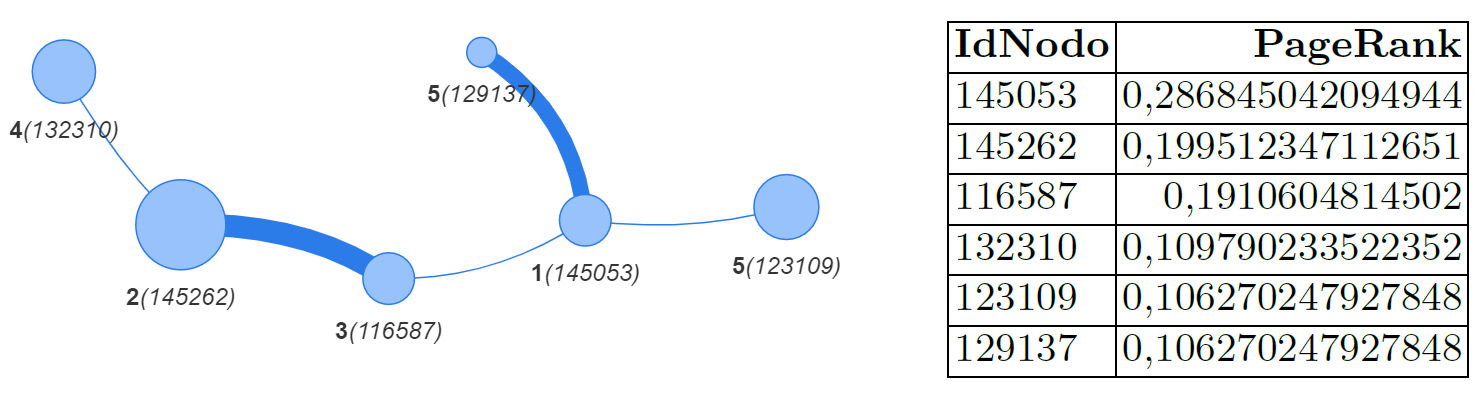
\includegraphics[width=0.50\linewidth]{6nodos-pageRank-sinColor-masTabla.png}
	\caption{Resultado de ejecución de PageRank para 6 nodos.} 
	\label{fig:6nodos-pageRank-sinColor-masTabla}
\end{figure}
%\vspace{-10pt}

Se ejecutó el algoritmo también para casos de estudio real resueltos en el MPF, donde las bandas y sus líderes han sido identificados, y de esta manera validar la relevancia de la implementación. Como ejemplo a continuación se muestra la Figura \ref{fig:BandaLCDs1}, sobre el caso real de robo de LCDs mencionado en el capítulo anterior. Pudo validarse que todos los integrantes de la banda se encuentran en el centro del subgrafo, altamente relacionados con los nodos de colores, que reflejan a los de más valor de PageRank.

\begin{figure}
	\centering
	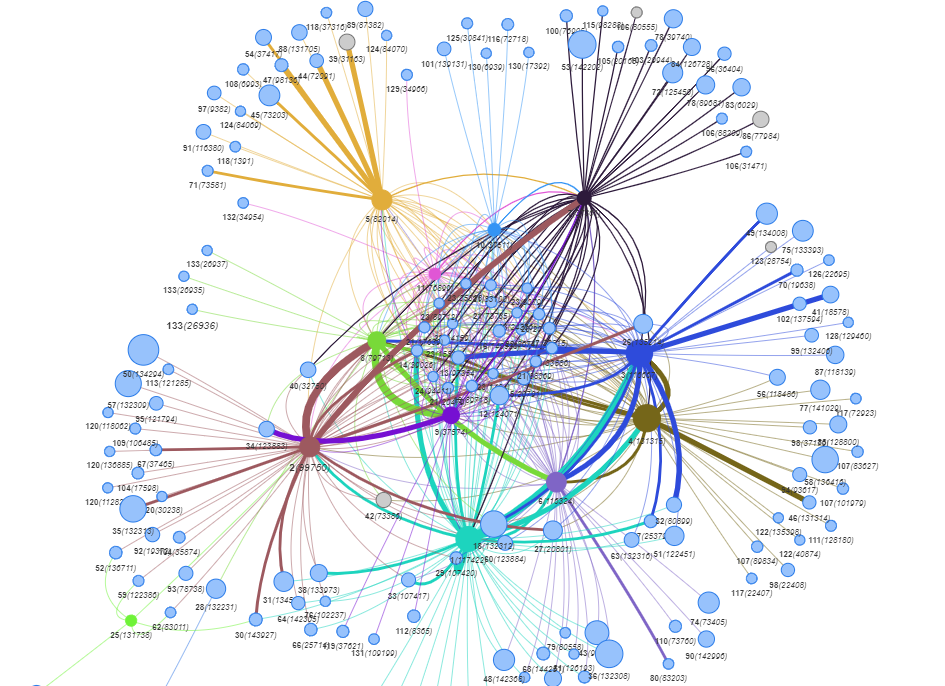
\includegraphics[width=0.40\linewidth]{BandaLCDs1.png}
	\caption{Resultado de ejecución de PageRank para el caso real de robo de LCDs.} 
	\label{fig:BandaLCDs1}
\end{figure}


%La visualización del grafo que combina información penal con la relevancia basada en la topología del grupo de pertenencia provee mayor asistencia a una identificación primaria de individuos de importancia.
%Esto es compatible con el patrón de comportamiento que indica que, en varias organizaciones delictivas, los líderes no siempre evidencian la mayor visibilización judicial, contrario a lo que ocurre en los estratos inferiores que están mas expuestos al delito cotidiano. Por ejemplo, en las estructuras de mafia siciliana el \textit{soldato} es quien realiza muchos de los actos delictivos simples de la Cosa Nostra, mientras que sus lideres los \textit{capo-decina} y \textit{capo-mandamento} se reservan mayor discreción. 



